% Antenna input impedance as a one-port: series R_rad, R_loss, jX, driven by a
% source through a feed line of impedance Z_0 (L4).
% Build: run scripts/circuits/build.sh -> book/extras/viz/img/antenna-input-z.svg
\documentclass[border=6pt]{standalone}
\usepackage{circuitikz}
\usetikzlibrary{arrows.meta}
\definecolor{navy}{HTML}{004A85}
\definecolor{cblue}{HTML}{0067B9}
\definecolor{camber}{HTML}{8A5A00}
\definecolor{cink3}{HTML}{5B6573}
\ctikzset{bipoles/thickness=1.1}
\begin{document}
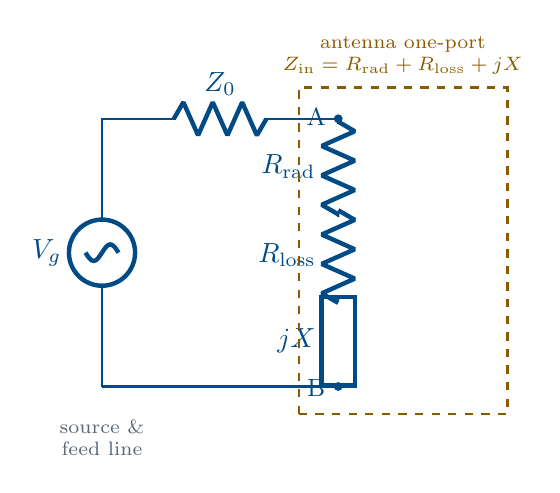
\begin{tikzpicture}[font=\sffamily, line width=0.8pt]
  % source + feed line on the left
  \draw[navy] (0,-1.7) to[sV, l=$V_g$, invert] (0,1.7) to[R, l=$Z_0$] (3,1.7);
  \draw[navy] (0,-1.7) -- (3,-1.7);
  \node[cink3, font=\scriptsize, align=center] at (0,-2.35){source \&\\ feed line};

  % antenna terminals A / B
  \fill[navy] (3,1.7) circle(1.6pt) (3,-1.7) circle(1.6pt);
  \node[navy, font=\small] at (2.72,1.72){A};
  \node[navy, font=\small] at (2.72,-1.72){B};

  % antenna branch: R_rad, R_loss, jX in series (labels to the right, inside box)
  \draw[navy] (3,1.7)
     to[R, l_=$R_\mathrm{rad}$]  (3,0.45)
     to[R, l_=$R_\mathrm{loss}$] (3,-0.55)
     to[generic, l_=$jX$]        (3,-1.7);

  % dashed box: the antenna one-port
  \draw[camber, dashed, line width=0.9pt] (2.5,-2.05) rectangle (5.15,2.1);
  \node[camber, font=\scriptsize, align=center] at (3.82,2.5)
        {antenna one-port\\ $Z_\mathrm{in}=R_\mathrm{rad}+R_\mathrm{loss}+jX$};
\end{tikzpicture}
\end{document}
